% main.tex — esqueleto del manuscrito (ángulo A: la curva harness-vs-escala).
%
% Venue aún por decidir (candidatos: TMLR, EMSE — ver discusión 2026-07-10);
% article genérico portable: migrar al template del venue al decidir.
% Compilar: make  (o pdflatex main && bibtex main && pdflatex ×2)
%
% Estado: ESQUELETO con contenido real — números, figuras y claims salen de
% los docs de análisis commiteados (citados en % comentarios por sección).
% Los TODO marcan prosa por escribir o datos por verificar.

\documentclass[11pt]{article}

\usepackage[utf8]{inputenc}
\usepackage[T1]{fontenc}
\usepackage[margin=1in]{geometry}
\usepackage{graphicx}
\usepackage{booktabs}
\usepackage{amsmath}
\usepackage[colorlinks=true, linkcolor=blue, citecolor=blue, urlcolor=blue]{hyperref}
\usepackage[round]{natbib}
\usepackage{xcolor}

\newcommand{\todo}[1]{\textcolor{red}{[TODO: #1]}}
\newcommand{\braze}{\textsc{braze}}

\title{The Harness Compensates the Model: A Pre-Registered Study of
Agentic Scaffolding Across Small-Model Scales%
\thanks{\todo{título candidato 1; alternativas: ``Not All Scaffolding
Helps: ...'' (enfatiza el resultado negativo), ``A 1B Agent That Beats
Its 7B Baseline: ...'' (enfatiza el dato estrella)}}}

\author{Francisco Parra\\
\todo{afiliación} \\
\texttt{\todo{email}}}

\date{}

\begin{document}
\maketitle

% =====================================================================
\begin{abstract}
% Fuente: docs/sweep-curva-multiescala-2026-07-10.md,
% docs/sweep-planner-ab-2026-07-11.md, docs/sweep-lead-3brazos-2026-07-10.md
Agentic coding harnesses are designed for frontier models; whether --- and
which --- scaffolding transfers to small, local models (1--8B) is largely
unmeasured. We present \braze{}, an open-source agentic harness built to
make that question measurable: every reliability lever is independently
switchable per benchmark row, every run is reproducible from a commit
hash and suite fingerprint, and design decisions were pre-registered
before their evaluations ran. Across 1{,}520 runs spanning four executor
scales and four harness configurations we find that a single capability
lever --- a small lead model that proactively opens each turn --- yields
+70\,pp pass rate at 1B, decaying monotonically to zero at the scale
ceiling; a 1B executor with this lever (89\%) outperforms 3B (68\%) and
7B (80\%) baselines. In contrast, a context lever (a prose plan injected
into the prompt) \emph{harms} at both extremes of the scale through a
single degeneration mode (empty responses). A pre-registered iteration
localizes the failure to the plan's \emph{delivery} --- rendered as the
assistant's own text --- and repairs it: re-rendered as user context it
gains +10\,pp on the strongest executor, and delivered as a typed task
list it gains +12\,pp on the smallest. We further isolate the lead's
mechanism experimentally (proactive opening, not reactive escalation)
and show that two-level tool deferral cuts prompt tokens $5.6\times$ at
no correctness cost. \todo{cerrar con 1 frase de takeaway para
practitioners.}
\end{abstract}

% =====================================================================
\section{Introduction}\label{sec:intro}
% Fuente: CLAUDE.md (tesis), PLAN.md, docs/SOTA-2026-07.md

\todo{párrafo 1 — el contexto: coding agents (Claude Code, Codex,
OpenCode, Goose) construidos alrededor de modelos frontier; el costo/
privacidad/latencia empujan hacia modelos locales chicos; la pregunta
abierta: ¿cuánto del harness transfiere?}

\todo{párrafo 2 — la tesis: el harness como variable que compensa la
escala del modelo. Antecedente directo: SWE-agent/ACI
\citep{yang2024sweagent} mostró que la interfaz agente-computadora mueve
el resultado tanto como el modelo; nosotros lo sistematizamos a través
de ESCALAS y con palancas conmutables una a una.}

\todo{párrafo 3 — por qué esto requiere infraestructura y no solo un
benchmark: ablations por fila, atribución causal, pre-registro.}

\paragraph{Contributions.}
\begin{enumerate}
  \item \textbf{The harness-vs-scale curve} (Fig.~\ref{fig:curva}):
    4 harness configurations $\times$ 4 executor scales, $n{=}95$ per
    cell, one binary. The capability lever decays monotonically
    (+70\,pp at 1B $\to$ $-4$\,pp at the ceiling); the context lever
    harms at both extremes via one degeneration mode.
  \item \textbf{Causal isolation of the dominant lever}: a three-arm
    experiment separating proactive opening from reactive escalation
    shows the entire gain comes from the former; the reactive trigger
    is structurally blind to the semantic failures that dominate
    (\S\ref{sec:mechanism}).
  \item \textbf{A negative result diagnosed and repaired under
    pre-registration} (Fig.~\ref{fig:rescate}): the planner's collapse
    (both extremes at 49\%) was a delivery bug, not a property of
    planning; the pre-registered iteration turns it into a
    scale-dependent gain (+10 to +12\,pp).
  \item \textbf{Cost-side levers quantified}: two-level tool deferral
    ($5.6\times$ fewer prompt tokens, no correctness cost,
    Fig.~\ref{fig:searchtools}); \todo{¿incluir colapso ACI/ablations
    acá o dejarlo en resultados secundarios?}
  \item \textbf{\braze{} itself}: an open-source Rust harness where
    every lever is a per-row benchmark ablation
    (\texttt{+ablate:\{no-rescue, no-prune, no-lead, task-list, ...\}}),
    releasable artifact with full sweep data. \todo{DOI Zenodo al
    empaquetar (/zenodo).}
\end{enumerate}

% =====================================================================
\section{Related Work}\label{sec:related}
% Fuente: docs/SOTA-2026-07.md; docs/opencode-a-braze.md;
% docs/harness-engineering-hooks-skills-2026-07-10.md

\paragraph{Agent-computer interfaces.} \todo{SWE-agent/ACI
\citep{yang2024sweagent}: la evidencia de que la interfaz importa; su
colapso de observaciones (+3pp SWE-bench Lite) es el antecedente del
colapso táctico de \braze{}. Nosotros: la dimensión escala.}

\paragraph{Small language models as agents.} \todo{Qwen3-Coder TR
\citep{qwen3coder}: overfitting al tool-template nativo — motiva los
hints proactivos por familia y el rescate textual. Survey de SLMs
\citep{todoSLMsurvey}: ICL débil y no-monotónico en modelos chicos —
motiva prompts cortos. arXiv 2604.02155 \citep{todoReasoningDegrades}:
razonamiento largo degrada tool-calling en modelos chicos.}

\paragraph{Multi-model orchestration.} \todo{Goose (lead/worker
reactivo) — nuestro A/B de 3 brazos muestra que la variante PROACTIVA
es la que paga; Aider architect/editor (+3-4pp) — calibra la ganancia
esperable del split planner/executor; best-of-n para tool-calling
\citep{corradini2025}.}

\paragraph{Agentic harnesses.} \todo{Claude Code / Codex / OpenCode /
Gemini CLI: principios de diseño (carga diferida, compactación
diferencial, permisos en capas) — no publicados como resultados
medibles; nuestra contribución es hacerlos conmutables y medirlos.}

% =====================================================================
\section{The \braze{} Harness}\label{sec:harness}
% Fuente: PLAN.md (arquitectura), CLAUDE.md (palancas)

\todo{descripción compacta: workspace Rust de 14 crates, tres traits
congelados (ToolProvider / ModelBackend / SessionStore+Compactor);
énfasis en que TODO lo demás es palanca conmutable.}

\begin{table}[t]
\centering\small
\caption{Reliability levers and their per-row benchmark ablations.
\todo{completar columna de default y sección de resultados donde se
mide cada una.}}
\label{tab:levers}
\begin{tabular}{llll}
\toprule
Lever & Mechanism & Ablation key & Measured in \\
\midrule
Lead model & proactive turn opening & \texttt{no-lead}, \texttt{lead-turns=N} & \S\ref{sec:curve},~\S\ref{sec:mechanism} \\
Planner & plan pre-round (3 deliveries) & \texttt{no-planner}, \texttt{task-list} & \S\ref{sec:planner} \\
Tool deferral & \texttt{search\_tools} meta-tool & \texttt{tool-search-threshold=N} & \S\ref{sec:searchtools} \\
Observation collapse & old tool outputs $\to$ 1 line & \texttt{no-prune}, \texttt{full-observations=N} & \todo{ablation sweep} \\
Textual rescue & per-family tool-call parsers & \texttt{no-rescue} & \todo{GLM vía OpenRouter} \\
Post-edit check & compiler feedback in-result & \texttt{no-post-edit-check} & \todo{ablation sweep} \\
Best-of-$n$ & vote among candidates & \texttt{best-of-n=N} & \todo{g10 sweep} \\
Harness notes & budget/deadline warnings & \texttt{no-harness-notes} & \todo{pendiente} \\
Typed task list & plan as state, compact re-injection & \texttt{task-list} & \S\ref{sec:planner} \\
\bottomrule
\end{tabular}
\end{table}

% =====================================================================
\section{Experimental Setup}\label{sec:setup}
% Fuente: braze-bench (diseño), docs de sweeps (metadata)

\todo{suite (19 tareas, 5 skills: single\_tool / no\_tool / multi\_step /
error\_recovery / distractor\_selection), sandbox por corrida, timeout,
5 repeticiones, temp 0.2; modelos (llama3.2:1b, qwen2.5:3b/7b,
qwen3.5-coder; gemma4:e4b como lead/planner fijo); nodo de inferencia
dedicado (regla un-sweep-a-la-vez tras medir contaminación).}

\paragraph{Reproducibility.} Every sweep JSON embeds the harness git
commit, a suite fingerprint, and per-model digests; confidence
intervals are 95\% Wilson ($n{=}95$ per cell unless noted); deltas
across sweeps are never compared as levels, only within-sweep
(Newcombe/MOVER intervals for differences). \todo{párrafo sobre
pre-registro: criterios del planner y del explorador escritos antes de
sus sweeps, citables por commit.}

% =====================================================================
\section{Results}\label{sec:results}

\subsection{The harness-vs-scale curve}\label{sec:curve}
% Fuente: docs/sweep-curva-multiescala-2026-07-10.md

\begin{figure}[t]
  \centering
  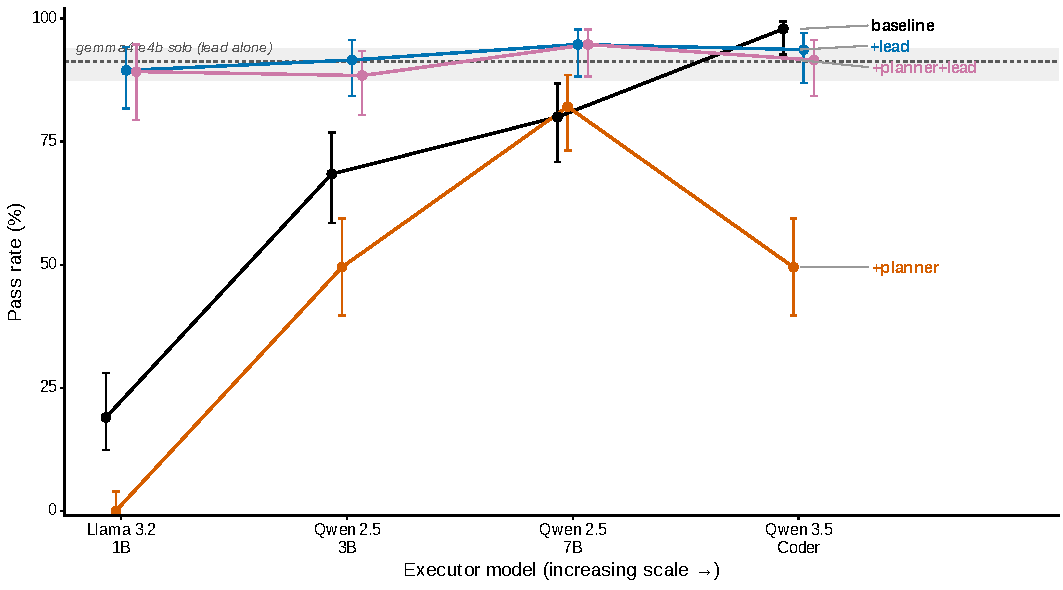
\includegraphics[width=\linewidth]{figs/fig1_curva.pdf}
  % Caption sugerido (el título va acá, nunca dentro de la figura):
\caption{Harness-versus-scale curve. Pass rate on the 19-task suite
(5 repetitions, $n{=}95$ per cell; error bars are 95\% Wilson
confidence intervals) for four
executor models of increasing scale, under four harness
configurations: no scaffolding (baseline), a planning pre-round whose
prose plan enters the context (+planner), a capable lead model that
proactively opens each turn (+lead, gemma4:e4b), and their
composition. The shaded band and dashed line
mark \texttt{gemma4:e4b}'s own solo pass rate (91.2\% [87.4, 94.0]\%,
pooled $n{=}285$, pre-registered baseline): the \texttt{+lead} line
sits inside that band at every executor scale, never distinguishably
above it (a same-batch, within-discipline comparison at 1B; at the
other three scales a cross-sweep juxtaposition offered as visual
context --- see Section~\ref{sec:curve}), so the lead's apparent gain
($+70$\,pp at 1B, $-4$\,pp at
the ceiling) is a roughly constant composite --- the lead's own
ceiling --- minus a baseline that rises with scale, and a 1B executor
with a lead (89\%) outperforming the 3B (68\%) and 7B (80\%) baselines
is better read as the lead's capability routed efficiently than as an
emergent property of the composition
(Section~\ref{sec:curve}). The prose plan \emph{harms} at both
extremes of the scale through the same empty-response degeneration
mode, diagnosed in Section~\ref{sec:planner} --- yet the
\texttt{+planner+lead} line tracks \texttt{+lead} at every scale, so
the lead absorbs that damage entirely once it opens the turn. The
composed cell at 1B is plotted from its pre-registered clean re-run
(2026-07-19, $n{=}95$, zero transport failures: 88.4\%), which
replaced a transport-contaminated original measurement --- provenance,
history, and the within-sweep delta against its own anchor arm
($+0.0$\,pp) in Section~\ref{sec:curve}.}

  \label{fig:curva}
\end{figure}

\todo{prosa de los 6 hallazgos del doc de la curva: (1) decaimiento
monótono del lead +70/+24/+15/-4pp y el dato estrella 1B+lead 89\% >
7B baseline 80\%; (2) el planner-prosa colapsa ambos extremos por
respuestas vacías (37 y 35 de las fallas); (3) la composición hereda el
gradiente; (4) la excepción informativa del 7B; (5) en el techo +lead
es MÁS RÁPIDO que baseline (19.8 vs 23.7s); (6) replicaciones del 3b en
la banda 67-72\% a través de 4 sweeps.}

\subsection{Isolating the mechanism: proactive opening, not reactive
escalation}\label{sec:mechanism}
% Fuente: docs/sweep-lead-3brazos-2026-07-10.md

\todo{el A/B de 3 brazos: proactivo 92.6\% [85.6,96.4] vs reactivo puro
75.8\% [66.3,83.3] vs baseline 67.4\%; las 13 fallas de error\_recovery
del brazo reactivo con CERO escalaciones — el trigger (tool failures
consecutivas) es estructuralmente ciego a ``ejecutar con éxito la
acción equivocada''; cuando dispara, 7/7 pasan. Lección: mecanismo
válido, cobertura estrecha.}

\subsection{A negative result, diagnosed and repaired}\label{sec:planner}
% Fuente: docs/sweep-planner-ab-2026-07-11.md; docs/sweep-matriz-4brazos-2026-07-10.md

\begin{figure}[t]
  \centering
  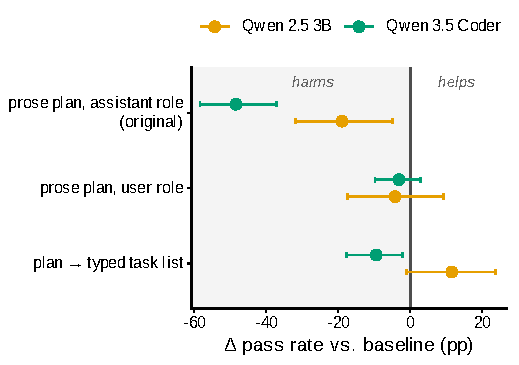
\includegraphics[width=0.6\linewidth]{figs/fig2_rescate.pdf}
  % Caption sugerido:
\caption{Rescuing the planner: the delivery format, not the plan,
caused the collapse. Change in pass rate relative to the same-sweep
baseline (percentage points; error bars are 95\% Newcombe/MOVER
intervals over Wilson bounds) for three deliveries of the same
planning pre-round. Rendering the plan as the \emph{assistant's own}
text (original design) collapses both executors through empty-response
degeneration; re-rendering it as \emph{user} context restores the
capable executor to its baseline ($-3.2$\,pp [$-9.8$, $+2.9$], no
demonstrable gain), while delivering it as a typed task list
re-injected compactly each round yields the largest movement,
$+11.6$\,pp on the small executor (95\% interval [$-1.0$, $+23.7$],
marginally crossing zero) --- but lands measurably \emph{below}
baseline on the capable one ($-9.5$\,pp [$-17.6$, $-2.2$];
Section~\ref{sec:planner} reports the committed criterion's literal
verdict). The original arms were measured in
the scale sweep ($n{=}95$ per arm); the capable executor's fixed
deliveries and baseline come from a pre-registered clean re-run
($n{=}95$ per arm, zero transport failures), the small executor's from
the follow-up A/B net of a disclosed transport event (its task-list
arm is a clean re-run); all deltas are within-sweep
(Section~\ref{sec:planner}).}

  \label{fig:rescate}
\end{figure}

\todo{la secuencia completa como narrativa de método: (1) A/B original
negativo $\to$ queda opt-in con iteración pre-registrada; (2) la matriz
lo vuelve decisivo (-22pp, degeneración diagnosticada); (3) la curva
muestra el mismo modo en ambos extremos; (4) la iteración (render
user-role + descarte single-step + entrega como task list) rescata:
prosa-user +10pp en coder, task-list +12pp en 3b; (5) el criterio
pre-registrado impidió tanto el falso rechazo como el rescate ad-hoc.
Nota del brazo contaminado y su re-run (transparencia).}

\subsection{Tool deferral: cost, not correctness}\label{sec:searchtools}
% Fuente: docs/sweep-search-tools-ab-2026-07-11.md

\begin{figure}[t]
  \centering
  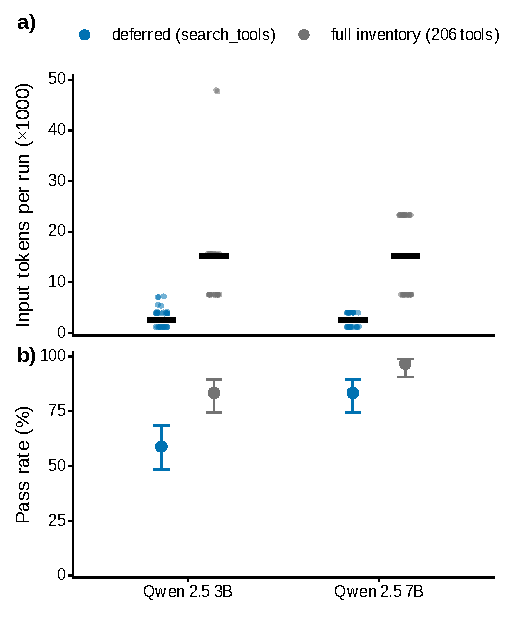
\includegraphics[width=0.6\linewidth]{figs/fig3_search_tools.pdf}
  % Caption sugerido:
\caption{Two-level tool deferral: same correctness, $5.6\times$ fewer
prompt tokens. On a suite whose tasks require only the six local tools
but whose registry carries 200 synthetic noise tools (an MCP-gateway
stand-in), hiding the noise catalog behind a single \texttt{search\_tools}
meta-tool (blue) versus listing all 206 tools (grey).
\textbf{(a)}~Input tokens per run (points: individual runs, $n{=}30$
per arm; black bar: median). \textbf{(b)}~Pass rate (95\% Wilson CIs).
Correctness is unchanged (7B) or within noise (3B) — the models are
not measurably distracted by 200 irrelevant tools — while prompt cost
collapses $5.6\times$ and wall-clock roughly halves (not shown). At
the scale of real tool gateways (1{,}500+ tools) the full-inventory
arm would exceed the local context window outright: deferral is
enabling, not merely cheaper.}

  \label{fig:searchtools}
\end{figure}

\todo{honestidad primero: la hipótesis de distracción NO se confirmó a
200 tools de ruido — la cantidad no distrae, la plausibilidad sí
(contraste con distractor\_selection). La ganancia es costo: 5.6× tokens,
2.4× wall; a escala gateway (1500+) es habilitación.}

\subsection{Secondary levers and ablations}\label{sec:ablations}
\todo{qué entra acá: rescued\_tool\_calls=0 en 665 corridas con Qwen
(el rescate no dispara donde no hay leak — honestidad sobre una palanca
estrella que no se activó en este régimen; SÍ se activa con GLM vía
OpenRouter, citar evidencia U-15/U-16); ¿correr ablation sweep de
no-prune/post-edit-check para esta sección o declararlo future work?}

% =====================================================================
\section{Discussion}\label{sec:discussion}

\todo{(1) Not all scaffolding helps: palancas de CAPACIDAD en rounds
tempranos suman; palancas de CONTEXTO restan salvo entrega correcta —
y la entrega correcta depende de la escala (prosa para capaces, estado
tipado para chicos). (2) El harness le debe avisos al modelo chico
(deadline anunciado vs corte silencioso). (3) Pre-registro como
disciplina de ingeniería, no solo de ciencia: dos veces evitó
decisiones equivocadas. (4) Implicación práctica: un 1B con lead barato
como configuración edge viable.}

\section{Threats to Validity}\label{sec:threats}
\todo{(1) suite propia de 19 tareas — mitigación pendiente: anclar con
benchmark externo (BFCL subset) o suite ampliada; (2) un solo
lead/planner (gemma4:e4b); (3) n=15 por celda de skill (solo extremos
concluyentes); (4) modelos de una familia dominante (Qwen) + 1
Llama; (5) fallos transitorios de infraestructura documentados y
excluidos/re-corridos con transparencia (listar los 3 casos).}
% --- Caveats de la auditoría v7 (docs/AUDITORIA-2026-07-v7.md) que esta
% sección debe declarar sobre los sweeps YA corridos (los fixes están en
% el código, pero los JSON citados son pre-fix):
% J-10/J-21: tokens y rondas de filas Timeout son cota inferior (la
%   ronda en vuelo se pierde al cortar) — las comparaciones de costo
%   entre brazos con distinta tasa de timeout favorecen al brazo que más
%   falla. Declarar, o comparar solo sobre filas convergidas.
% J-17: el brazo con deferral (Fig. 3) corrió con un budget de contexto
%   calculado sobre el catálogo COMPLETO pre-deferral — sesgo CONTRA el
%   brazo search_tools (compactaba antes de lo necesario): el 5.6× es
%   conservador, no inflado.
% J-6: los sweeps pre-fix no tenían warm-up por brazo — posible sesgo de
%   wall-time a favor de brazos tardíos bajo --no-ollama-stop; no afecta
%   pass rates salvo timeouts en la primera tarea del primer brazo.
% J-2: RESUELTO CON RE-RUN (docs/sweep-planlead-taskslead-postfix-2026-07-11.md):
%   en el sweep original el resumen de la task list reseteaba la racha de
%   fallos del EscalatingBackend (escalación reactiva muerta en el brazo
%   tasks+lead). El re-run controlado post-fix (190 corridas, ancla
%   incluida) muestra 9 escalaciones reactivas reales y el MISMO
%   veredicto: tasks+lead 83.2% vs lead solo 92.6% (ancla en su banda
%   92-92.6% por 5ª vez). "Tasks+lead resta" es interferencia real de
%   andamiajes, no el artefacto — citar el re-run como control.
% J-7: expect_text_contains evaluaba TODO el texto del turno (narración
%   pre-tool-call incluida) — posibles falsos PASS direccionales hacia
%   modelos verbosos; las celdas apretadas deberían re-verificarse con
%   el fix si se citan a nivel de skill.

\section{Conclusion}\label{sec:conclusion}
\todo{1 párrafo: la curva existe, tiene mecanismo, y sus excepciones
tienen diagnóstico. El harness compensa escala — pero solo el andamiaje
correcto, entregado en el formato correcto para la escala.}

% =====================================================================
\paragraph{Artifact availability.} \todo{repo + DOI Zenodo del código y
los 8 sweep JSONs (~4.400 corridas totales citadas); instrucciones de
reproducción por sweep están en cada docs/sweep-*.md.}

\bibliographystyle{plainnat}
\bibliography{refs}

\appendix
\section{Sweep inventory}\label{app:sweeps}
\todo{tabla: cada sweep citado, su commit, n, fecha, archivo JSON — la
fuente es el encabezado de cada docs/sweep-*.md.}

\section{Pre-registration texts}\label{app:prereg}
\todo{transcribir los dos pre-registros con su commit: el criterio del
planner (PLAN.md, previo al A/B) y el diseño del explorador
(docs/explorador-aislado-ab-design.md) como ejemplo de la disciplina
aplicada a futuro.}

\end{document}
